% !TEX root = ../main.tex
\section{Quantization-Aligned Caching}
\label{sec:qac}

\subsection{Decision-Domain Mismatch}
Let $F_t$ denote the low-cost feature observed by the cache controller before the expensive STDiT execution at denoising step $t$. Conventional timestep caching, such as TeaCache~\cite{liu2025teacache}, measures its normalized full-precision (FP) variation,
\begin{equation}
 d_t^{\mathrm{FP}}=
 \frac{\lVert F_t-F_{t-1}\rVert_1}
      {\lVert F_{t-1}\rVert_1+\epsilon}.
 \label{eq:fp_indicator}
\end{equation}
The predictor is therefore calibrated on an FP trajectory, whereas every recomputed step in our target pipeline follows fixed W8A8/INT8 execution. Quantization is nonlinear and piecewise constant: two nearby FP values may collapse to the same integer code, while a smaller FP change may cross a quantization boundary and alter the executed representation. Hence $d_t^{\mathrm{FP}}$ need not preserve the relative importance of recomputation after quantization. This is not merely a scalar bias that can be removed by rescaling the FP indicator. Because the cache rule accumulates predicted variation and triggers recomputation on a threshold crossing, such reordering can change both which steps are reused and when the cached state is refreshed. We call this the \emph{decision-domain mismatch}.

\subsection{Quantization-Aligned Indicator}
QAC evaluates cache relevance in the same numerical domain as the recompute path. With the frozen activation scale $s$, it forms
\begin{equation}
 \widetilde F_t=D(Q_s(F_t)),\qquad
 d_t^{\mathrm Q}=
 \frac{\lVert\widetilde F_t-\widetilde F_{t-1}\rVert_1}
      {\lVert\widetilde F_{t-1}\rVert_1+\epsilon},
 \label{eq:q_indicator}
\end{equation}
where $Q_s(\cdot)$ and $D(\cdot)$ denote quantization and dequantization. The same calibrated quantizer is therefore used both to execute the model and to determine whether execution is needed, exposing the cache predictor to the same rounding and clipping effects as the recomputed path. QAC changes the decision domain without introducing another precision mode; all recomputed GEMMs and attention operators remain on the fixed W8A8/INT8 datapath.

\begin{figure*}[!t]
  \centering
  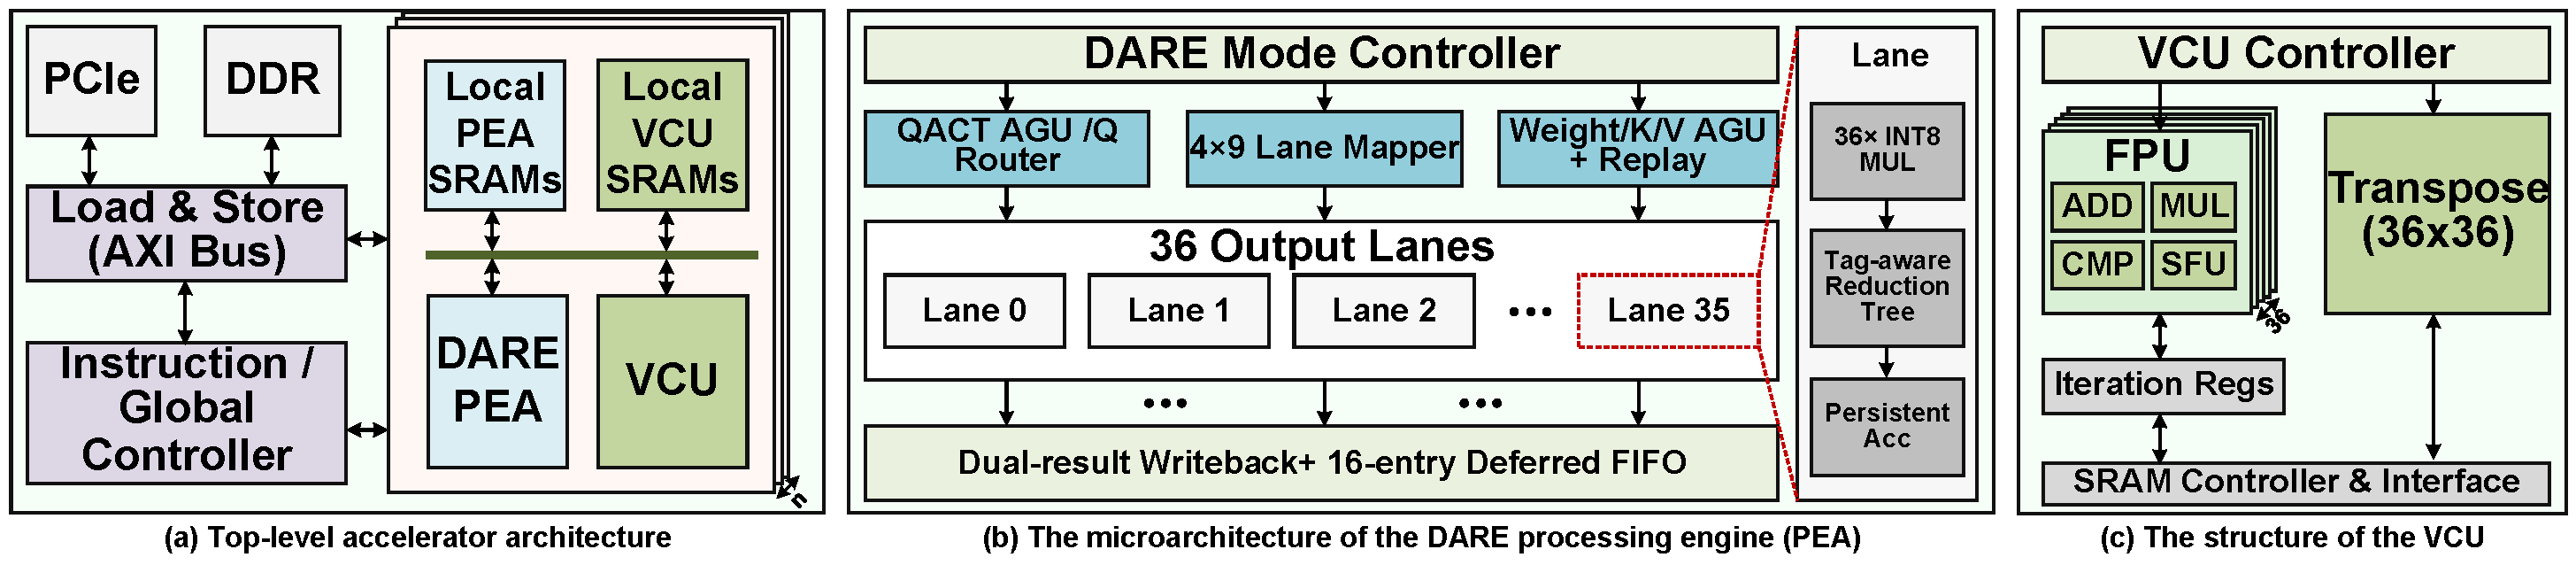
\includegraphics[width=\textwidth]{fig/hardware-overview.pdf}
  \caption{DARE hardware organization: (a) Top-level accelerator architecture; (b) The microarchitecture of the DARE PEA; and (c) the structure of the VCU.}
  \label{fig:dare_arch}
\end{figure*}

\subsection{Calibration and Runtime Policy}
The raw quantized-domain difference is further calibrated against the observed output change of the quantized model. Offline, QAC fits a lightweight timestep-aware mapping
\begin{equation}
 \widehat r_t^{\mathrm Q}=g_q(d_t^{\mathrm Q},t),
 \label{eq:qac_mapping}
\end{equation}
where the timestep input captures the varying sensitivity of the denoising trajectory. Because $g_q$ is fitted to quantized output variation rather than a binary cache label, it remains compatible with the accumulated reuse budget instead of hard-coding a fixed cache schedule. This is useful across denoising, where the same feature-change magnitude can have different consequences at different timesteps.

At runtime, QAC computes $d_t^{\mathrm Q}$ before STDiT execution, evaluates $g_q$, and feeds the predicted change to the baseline thresholded cache rule. Cached states are reused while accumulated predicted variation remains within the reuse budget; once the budget is exceeded, STDiT is recomputed and the cached state is refreshed. Thus QAC calibrates the indicator without replacing the original cache semantics. At the hardware boundary it emits only a cache/recompute decision: a recompute request enters the same W8A8/INT8 path accelerated by DARE, requiring neither an FP side path nor a new PEA arithmetic mode.
